\chapter{Risultati}
In questo capitolo saranno presentati i risultati ottenuti nelle varie
simulazioni. Quando non meglio specificato, i parametri sono stati mantenuti
come indicato nel capitolo relativo alla progettazione.\newline
Visto il nostro assegnamento dei valori di fitness, il punteggio massimo è 100
punti, ottenuto non entrando mai nei muri, non scontrandosi mai con altri robot
e raccogliendo tutte e 10 le lattine.



\section{Entità Invisibili - Vista a Croce}

\subsection{100 Coppie, 0 Vecchi}
La prima simulazione è stata effettuata usando lo schema dell'algoritmo genetico
descritto precedentemente, con un numero di coppie pari a 100, ovvero 200 robot.
In 5000 generazioni il valore di fitness, dopo un primo incremento, si è sempre
mantenuto attorno al valore 0. Questo ci ha fatto supporre che la strategia di
evoluzione da noi adottata dovesse essere modificata. Anziché generare tutti i
nuovi individui mediante l'utilizzo del crossover, abbiamo deciso di copiare
alcuni degli individui vecchi nella nuova generazione, adottando una strategia
élitaria.

\subsection{100 Coppie, da 1 a 5 Vecchi}
\begin{figure}[ht]
	\centering
	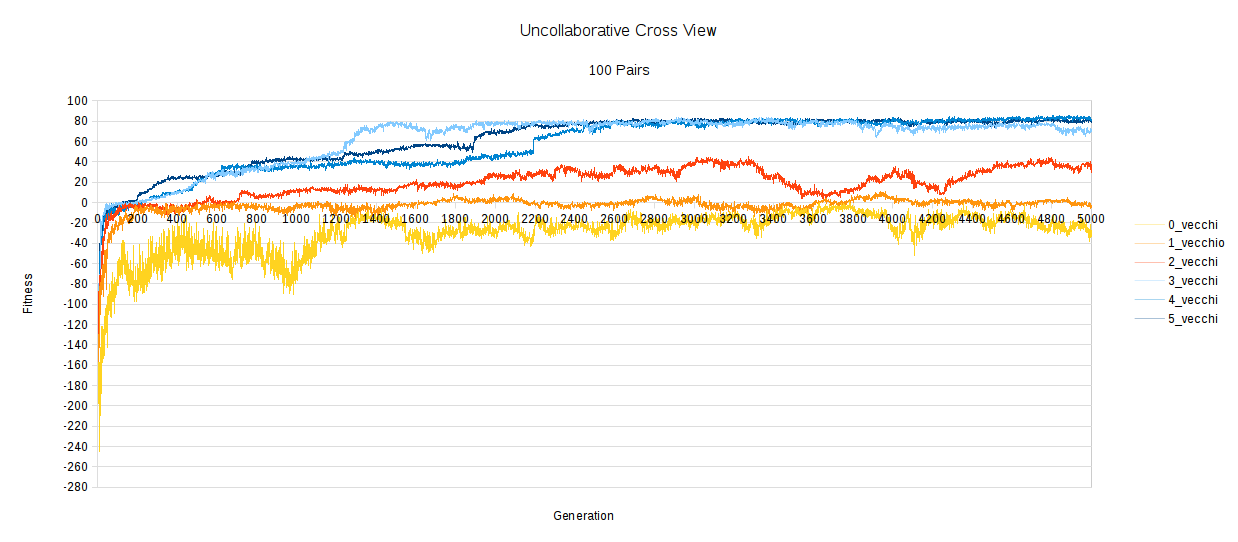
\includegraphics[scale=0.7,angle=90]{imgs/uncollaborative_cross_100_pairs_0_5_vecchi.png}
	\caption{Vista a croce non collaborativa, 100 coppie}
	\label{figure:uncoll_cross_100_0_5}
\end{figure}
La Figura~\ref{figure:uncoll_cross_100_0_5} mostra i valori di 6 simulazioni
nelle quali abbiamo mantenuto da 0 (tutti gli individui generati tramite l'uso
del crossover) a 5 coppie (le migliori) dalla vecchia alla nuova generazione.
Come è possibile notare, più sono gli individui che vengono mantenuti da una
generazione all'altra, più alto è il valore di fitness raggiunto.

\clearpage

\subsection{100 Coppie, da 10 a 35 Vecchie}
\begin{figure}[ht]
	\centering
	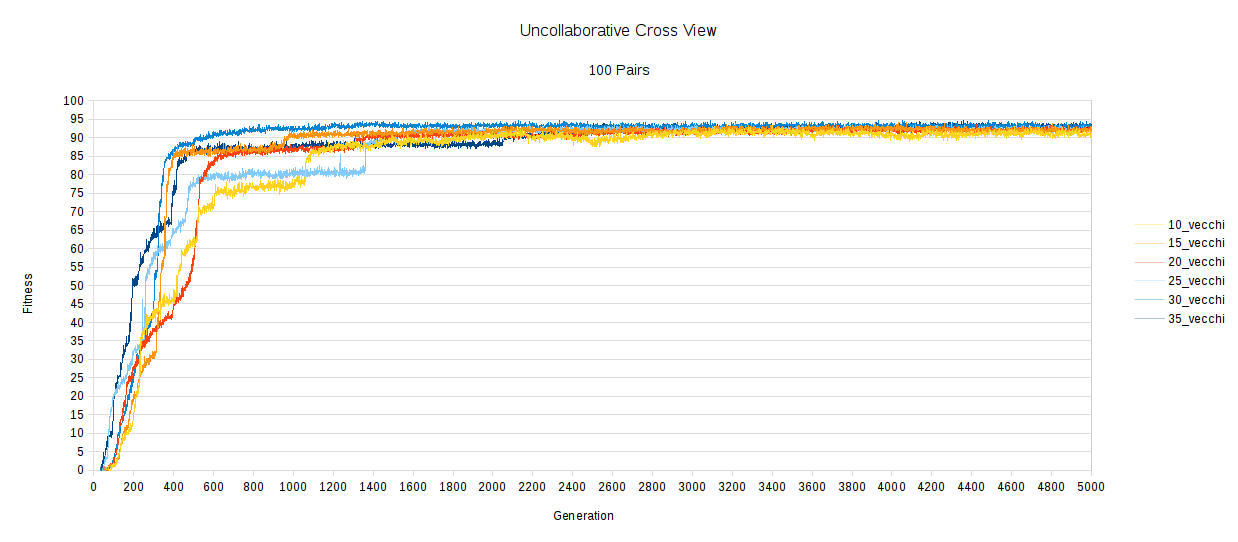
\includegraphics[scale=0.7,angle=90]{imgs/uncollaborative_cross_100_pairs_10_35_vecchi.png}
	\caption{Vista a croce non collaborativa, 100 coppie}
	\label{figure:uncoll_cross_100_10_35}
\end{figure}
In Figura~\ref{figure:uncoll_cross_100_10_35} abbiamo proseguito con il
ragionamento, copiando nella vecchia generazione da 10 a 35 coppie,
incrementando l'intervallo da 1 a 5. I valori di fitness si mantengono tutti fra
i 90 ed i 95 punti.

\subsection{100 Coppie, da 40 a 90 Vecchie}
\begin{figure}[ht]
	\centering
	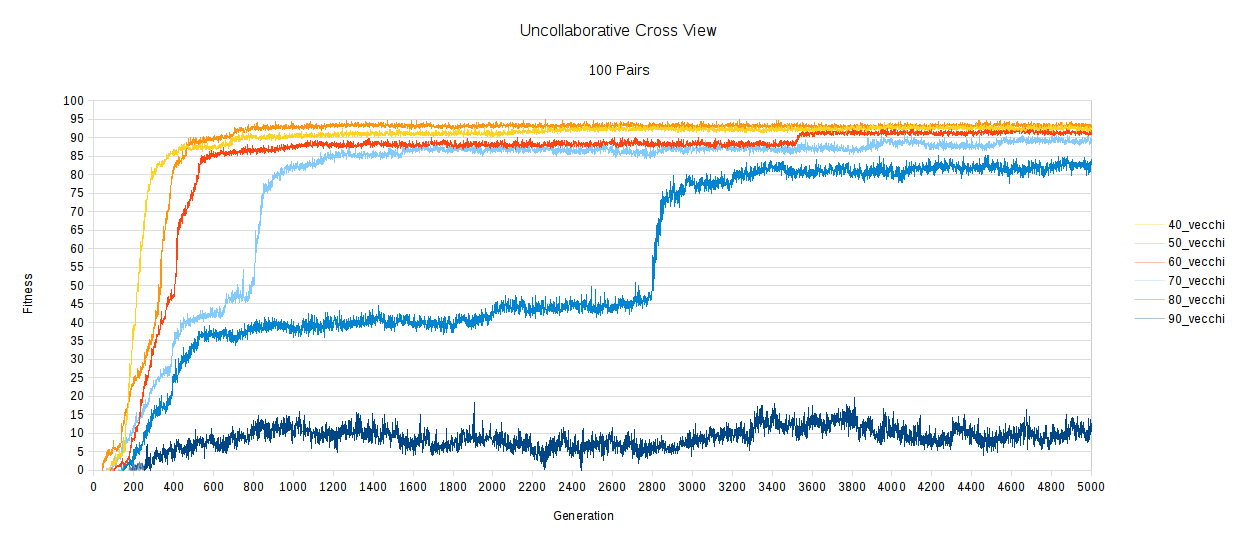
\includegraphics[scale=0.7,angle=90]{imgs/uncollaborative_cross_100_pairs_40_90_vecchi.png}
	\caption{Vista a croce non collaborativa, 100 coppie}
	\label{figure:uncoll_cross_100_40_90}
\end{figure}
A questo punto ci siamo chiesti quando le performance sarebbero crollate ed
abbiamo ulteriormente iterato il procedimento mantenendo da 40 a 90 coppie,
procedendo per intervalli di 10. Come è mostarto in Figura
\ref{figure:uncoll_cross_100_40_90}, man mano che il numero di coppie vecchie
passate nella nuova generazione aumenta, il valore di fitness inizia a scendere,
fino a mostrare cali importanti con 80 e 90 coppie. Mantenendo nella nuova
generazione 40, 50 e 60 coppie, comunque i valori di fitness rimangono fra i 90
ed i 95 punti.

\subsection{200 Coppie, da 10 a 180 Vecchie}
\begin{figure}[ht]
	\centering
	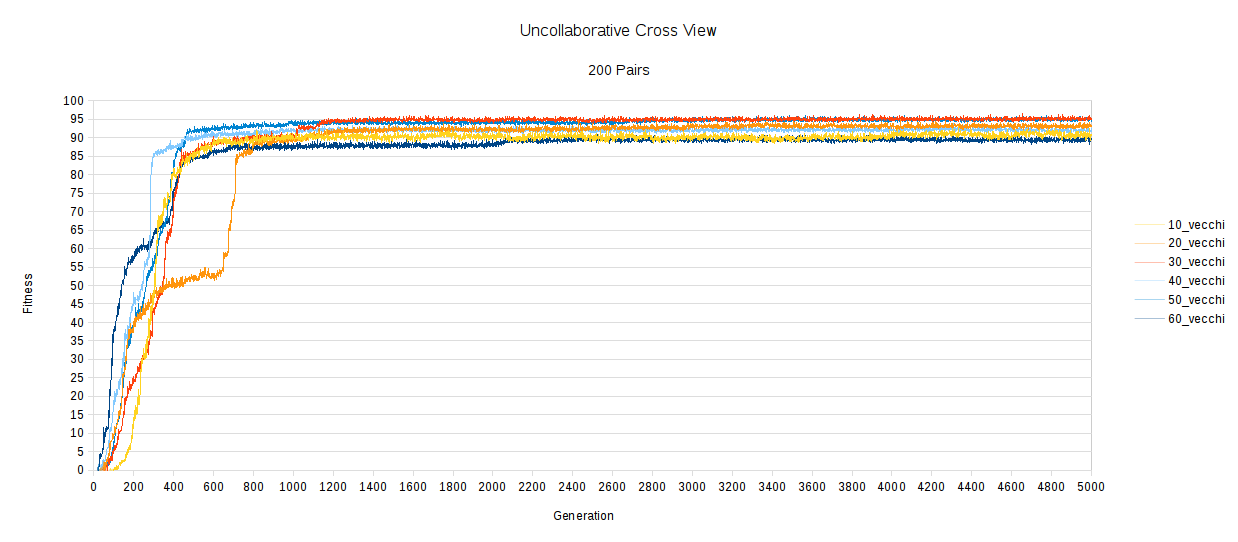
\includegraphics[scale=0.7,angle=90]{imgs/uncollaborative_cross_200_pairs_10_60_vecchi.png}
	\caption{Vista a croce non collaborativa, 200 coppie}
	\label{figure:uncoll_cross_200_10_60}
\end{figure}
\begin{figure}[ht]
	\centering
	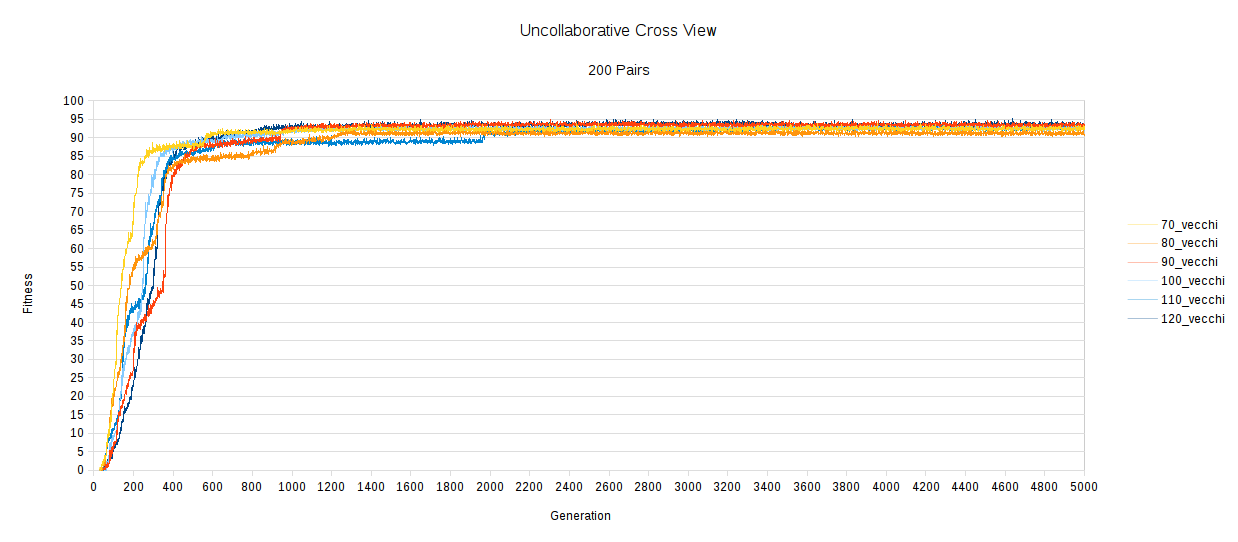
\includegraphics[scale=0.7,angle=90]{imgs/uncollaborative_cross_200_pairs_70_120_vecchi.png}
	\caption{Vista a croce non collaborativa, 200 coppie}
	\label{figure:uncoll_cross_200_70_120}
\end{figure}
\begin{figure}[ht]
	\centering
	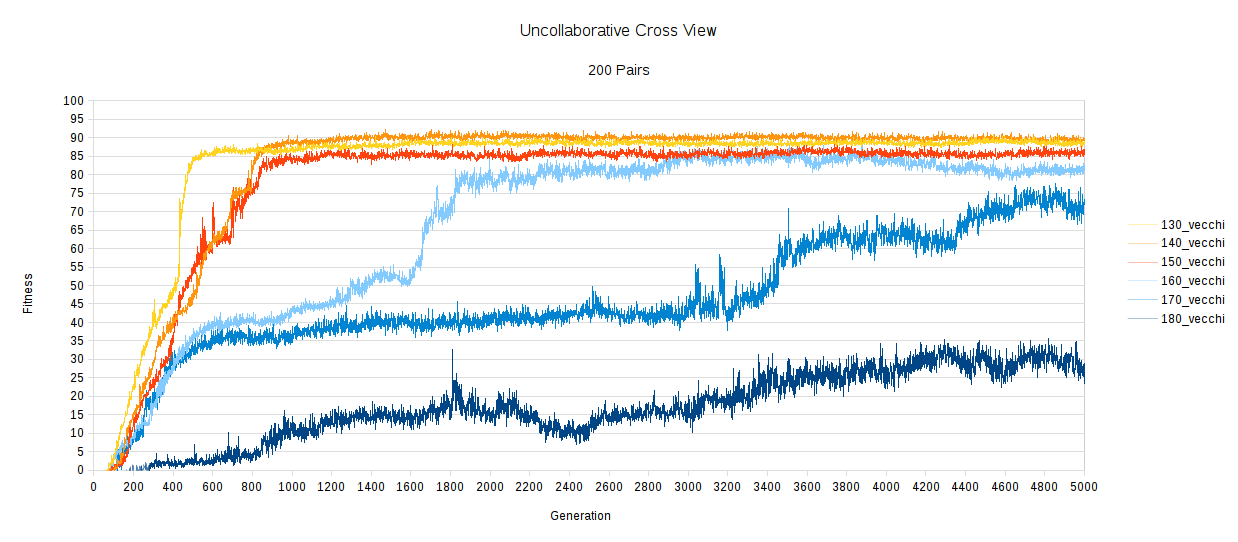
\includegraphics[scale=0.7,angle=90]{imgs/uncollaborative_cross_200_pairs_130_180_vecchi.png}
	\caption{Vista a croce non collaborativa, 200 coppie}
	\label{figure:uncoll_cross_200_130_180}
\end{figure}
Avendo notato come la modifica di un semplice parametro (il numero di coppie
vecchie da mantenere nella nuova popolazione) possa influenzare in maniera
significativa l'evoluzione, abbiamo deciso di ripetere lo stesso procedimento
aumentando il numero di coppie che formano la popolazione da 100 a 200. Così
facendo abbiamo sperato, avendo più varietà genetica all'inizio, di poter
raggiungere valori di fitness più alti.\newline
La Figura~\ref{figure:uncoll_cross_200_10_60} mostra l'andamento dell'evoluzione
tenendo da 10 a 60 coppie, la Figura~\ref{figure:uncoll_cross_200_70_120} da 70
a 120 e, infine, la Figura~\ref{figure:uncoll_cross_200_130_180} grafica
l'andamento dei valori di fitness tenendo da 130 a 180 coppie vecchie nella
nuova generazione.\newline
Per quanto riguarda il raggiungimento di valori di fitness più alti, partire
con una popolazione più grande (di dimensione doppia) non ha dato i risultati
sperati. Se però si notano le velocità con cui le varie curve crescono verso i
valori di fitness più grandi (il numero di generazioni che impiegano a superare,
ad esempio, gli 80/85 punti di fitness), ci si rende conto come avere una
popolazione formata da 200 coppie incrementi di molto le performance.\newline
Questo esperimento ci ha poi permesso di identificare una costante, ovvero, che
i valori di fitness più alti sono raggiunti mantenendo una percentuale
di coppie vecchie da una generazione all'altra che va dal 10\% al 60\%. Con una
popolazione di 100 coppie, infatti, i valori di fitness tra i 90 ed i 95 punti
sono stati raggiunti mantenendo da 10 a 60 vecchie coppie nelle nuove
generazioni, mentre, incrementando il numero di coppie a 200, gli stessi valori
di fitness sono raggiunti mantenendo da 20 a 120 vecchie coppie nelle nuove
generazioni.

\clearpage

\subsection{200 Coppie, da 70 a 120 Vecchie, Non Mutate}
\begin{figure}[ht]
	\centering
	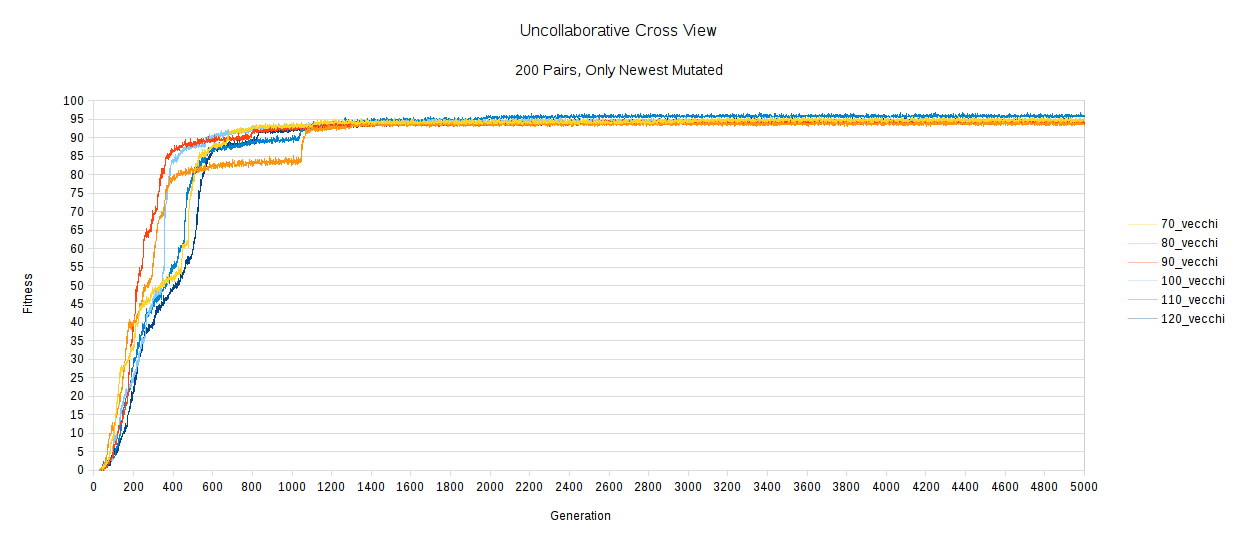
\includegraphics[scale=0.7,angle=90]{imgs/uncollaborative_cross_200_pairs_70_120_vecchi_solo_nuovi_mutati.png}
	\caption{Vista a croce non collaborativa, 200 coppie}
	\label{figure:uncoll_cross_200_70_120_vecchi_non_mutati}
\end{figure}
Abbiamo poi effettuato un'ultima simulazione nella quale abbiamo ripreso il
numero di coppie dalla vecchia alla nuova generazione che meglio si sono
comportate (che hanno raggiunto i valori di fitness più elevati) con popolazione
di dimensione 200 coppie, dove però le mutazioni genetiche sono state applicate
solo ai nuovi individui generati e non più anche ai vecchi.\newline
I risultati sono riportati in Figura
\ref{figure:uncoll_cross_200_70_120_vecchi_non_mutati}. Confrontando questo
grafico con quello di Figura~\ref{figure:uncoll_cross_200_70_120}, si nota come
la velocità nella crescita sia paragonabile ma, non mutando le vecchie coppie, i
valori di fitness siano tutti più elevati, non scendendo mai sotto i 95 punti
fitness.



\clearpage



\section{Entità Invisibili - Vista Quadrata}
